\documentclass{VUMIFPSbakalaurinis}
\usepackage{float}
\usepackage{hyperref}
\usepackage{algorithmicx}
\usepackage{algorithm}
\usepackage{algpseudocode}
\usepackage{amsfonts}
\usepackage{amsmath}
\usepackage{bm}
\usepackage{caption}
\usepackage{color}
\usepackage{graphicx}
\usepackage{listings}
\usepackage{subcaption}
\usepackage{wrapfig}
\usepackage{biblatex}
\usepackage{microtype}
\usepackage{mathtools}
\usepackage{multirow}

% Titulinio aprašas
\university{Vilniaus universitetss}
\faculty{Matematikos ir informatikos fakultetas}
\institute{Informatikos institutas}  % Užkomentavus šią eilutę - institutas neįtraukiamas į titulinį
\department{Programų sistemų bakalauro studijų programa}
\papertype{Laboratorinio darbo ataskaita}
\title{Perceptrono mokymas sprendžiant klasifikavimo uždavinį}
\titleineng{Artificial Neuron Model}
\author{Armintas Pakenis}
% \secondauthor{Vardonis Pavardonis}   % Pridėti antrą autorių
\supervisor{prof. dr. Olga Kurasova}
\reviewer{prof. dr. Olga Kurasova}
% \addsignatureplaces{} % prideda parašų vietas tituliniame puslapyje
\date{Vilnius – \the\year}

\bibliography{bibliografija}

\begin{document}
\maketitle

%% Padėkų skyrius
% \sectionnonumnocontent{}
% \vspace{7cm}
% \begin{center}
%     Padėkos asmenims ir/ar organizacijoms
% \end{center}

\tableofcontents

\section{Užduoties tikslas}
Užduoties tikslas — suprasti dirbtinio neurono modelį, 
jo veikimo principus ir tinkamai įgyvendinti jo mokymąsi dviejų klasių klasifikavimo uždaviniui.
Programoje naudotos bibliotekos: numpy ir matplotlib. Programos kodas rašytas Jupyter užrašų knygutės aplinkoje jį rasti galima GitHub repositorijoje: 
\href{https://github.com/ArmintasP/Computational-intelligence/tree/main/Lab2}{\color{cyan}{https://github.com/ArmintasP/Computational-intelligence/tree/main/Lab2}}.

\subsection{Duomenys}
Naudoti irisų duomenų ir krūties vėžio duomenų rinkiniai: 
\href{https://archive.ics.uci.edu/ml/datasets/iris}{\color{cyan}{https://archive.ics.uci.edu/ml/datasets/iris}}
ir
\href{https://archive.ics.uci.edu/ml/datasets/Breast+Cancer+Wisconsin+(Diagnostic)}{\color{cyan}{https://archive.ics.uci.edu/ml/datasets/Breast+Cancer+Wisconsin+(Diagnostic)}}.

Failai prieš mokymą apdoroti, pašalintos įeitys, turinčios trūkstančių požymių. 
Apdorotame irisų duomenų rinkinyje buvo 100, iš kurių po 50 įrašų kiekvienos klasės. Požymių skaičius — 4. 
Apdorotame krūties vėžio duomenų rinkinyje buvo 683, iš kurių po 239 priklausė vienai klasei, likusieji — kitai.
Požymių skaičius šiam rinkiniui — 10.

Įeičių tvarka prieš pradedant mokymą buvo sumaišyta, nes norėta išvengti tik vienos klasės įeičių mokymo rinkinyje.
80 procentų įeičių (kartu su trokštamomis reikšmėmis) buvo naudojami mokymo rinkinyje. Likusi dalis — validavimo rinkinyje.

\section{Perceptrono mokymas}
\subsection{Iteracijos ir epochos}
Epocha — mokymo proceso dalis, kuriuos metu apdorojamas mokymo ir validavimo įeičių rinkinys tik vieną kartą.
Šiame darbe duomenų rinkiniai nebuvo skaidomi į mažesnius rinkinius, 
iteracijų vienoje epochoje buvo tiek, kiek duomenų rinkinyje įrašų (100 ir 683).

\subsection{Pradiniai svoriai ir poslinkis}
Pradinės svorių reikšmės ir poslinkis buvo parenkami atsitiktinai, pagal Gauso skirstinį,
kitaip tariant, $ \mathbf{w} \sim \mathcal{N}(0, 1)$.
Mokymu metu svoriai buvo ieškomi pasitelkiant ADALINE mokymo taisyklę.


\section{Rezultatai}
Variantai, kada gaunami tiksliausi klasifikavimo rezultatai
ir mažiausia paklaida, su pateiktais svoriais, nuostolių funkcijų reikšmėmis,
epochų skaičiumi, klasifikavimo tikslumo įverčiais, bei kokias
klases identifiko perceptronas iš validavimo duomenų aibės
yra pateikti tekstiniuose failuose kiekvienam duomenų kiekiui
su skirtinga aktyvacijos funkcija repozitorijoje: \href{https://github.com/ArmintasP/Computational-intelligence/tree/main/Lab2/Results}
{\color{cyan}{https://github.com/ArmintasP/Computational-intelligence/tree/main/Lab2/Results}}.

Tiek treniravimo, tiek validavimo duomenims klasifikavimo tikslumas
didėja, jei epochų skaičius didėja. Be to,
matoma, jog dažnai validavimo rinkinio klasifikavimo tikslumas yra
mažesnis nei treniravimo. Tai matyti iš visų žėmiau
esančių paveikslėlių su grafikais
(žr. \ref{img:cancer-sigmoid}, \ref{img:cancer-heaviside},
\ref{img:iris-sigmoid}, \ref{img:iris-heaviside} paveikslėlius).
Tačiau galima pastebėti, kad esant dideliam epochų skaičiui,
modelis persimoko. Pavyzdžiui, \ref{img:iris-sigmoid} ir
\ref{img:iris-heaviside} paveikslėliuose matyti, kad 
nuo 40 epochos klasifikavimo tikslumas tampa nebe stabilus,
įgyja net mažesnes reikšmes už pasiektas anksčiau. 


Tiek treniravimo, tiek validavimo duomenims nuostolių funkcijos
reikšmė mažėja, jei epochų skaičius didėja. Neintuityviai gali atrodyti,
jog validavimo duomenims nuostolių funkcija turi daug mažesnes reikšmes
nei trenravimo duomenys. Taip atsitinka todėl, kad validavimo duomenų
turime mažiau ir naudojame vidutinę paklaidos funkciją 
$\frac{1}{2} \sum_{i=1}^{n}(x_i-y_i)^2$.
Egzistuoja ta pati problema kaip su klasifikavimo tikslumu —
didėjant epochų skaičiui, didėja tikimybė modeliui persimokyti.
Tai labiausiai galime pamatyti \ref{img:iris-sigmoid} ir\ref{img:iris-heaviside} paveikslėliuose
paveikslėliuose, kur nuo 60 epochos modelis persimoko.


Krūties vėžio duomenų aibė daug jautresnė modelio persimokymui lyginant
su irisų duomenų aibę. Taip yra todėl, kad dėl krūties vėžio duomenys
turi daugiau požymių ir turime bent 6 kartus daugiau įrašų.


Toliau aptariant minėtus grafikus, ženklaus pranašumo
tarp sigmoidinės ir slenkstinės aktyvacijos funkcijų nematyti.
Tiesa, panašu, kad su mažesniu duomenų rinkiniu sigmoidine funkcija
yra stabilesnė nei slenkstinė (žr. \ref{img:iris-sigmoid} ir ir\ref{img:iris-heaviside}
paveikslėlius).

Aiškios tendencijos tarp mokymosi greičio ir nuostolių funkcijos reikšmių ar 
klasifikavimo tikslumo su duotais rinkiniais nėra (žr. \ref{tab:e-100-cancer-sig},
\ref{tab:e-10-cancer-sig}, \ref{tab:e-100-iris-sig}, \ref{tab:e-10-iris-sig} lenteles ).
Tiesa, irisų duomenų rinkinys turėjo didesnį skirstumą tarp treniravimo ir validavimo
duomenų rinkinių, kai buvo skirtingi mokymosi greičiai.


\begin{figure}[H]
  \centering
  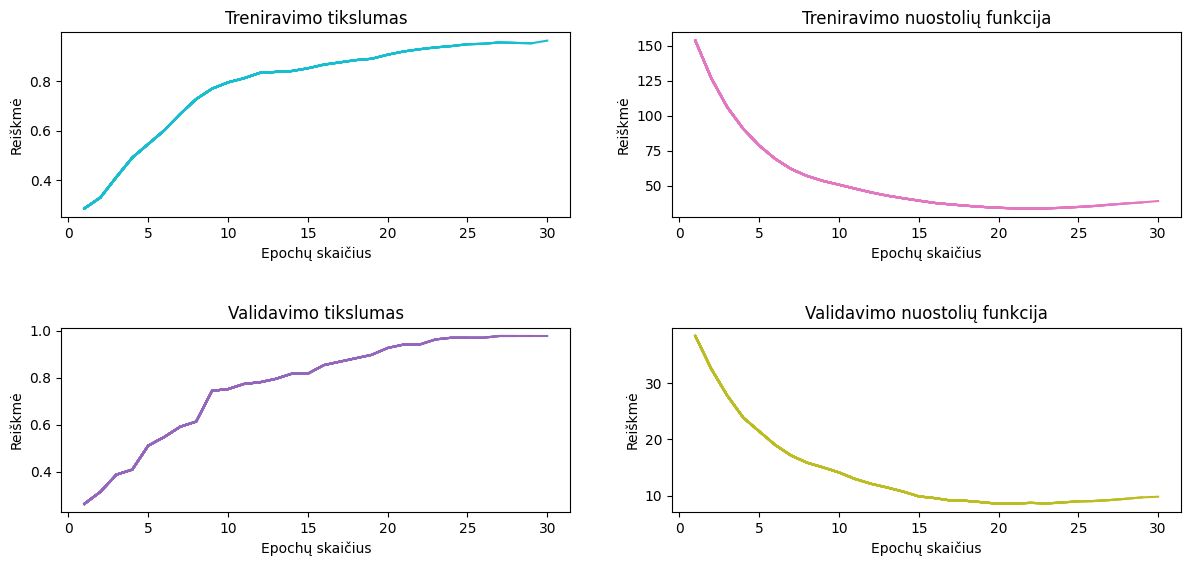
\includegraphics[scale=0.5]{img/1.png}
  \caption{Perceptrono mokymas naudojant krūties vėžio
   duomenų rinkinį ir sigmoidinę aktyvacijos funkciją.
   Epochų skaičius: 30, mokymosi greitis: 0,001}
  \label{img:cancer-sigmoid}
\end{figure}

\begin{figure}[H]
  \centering
  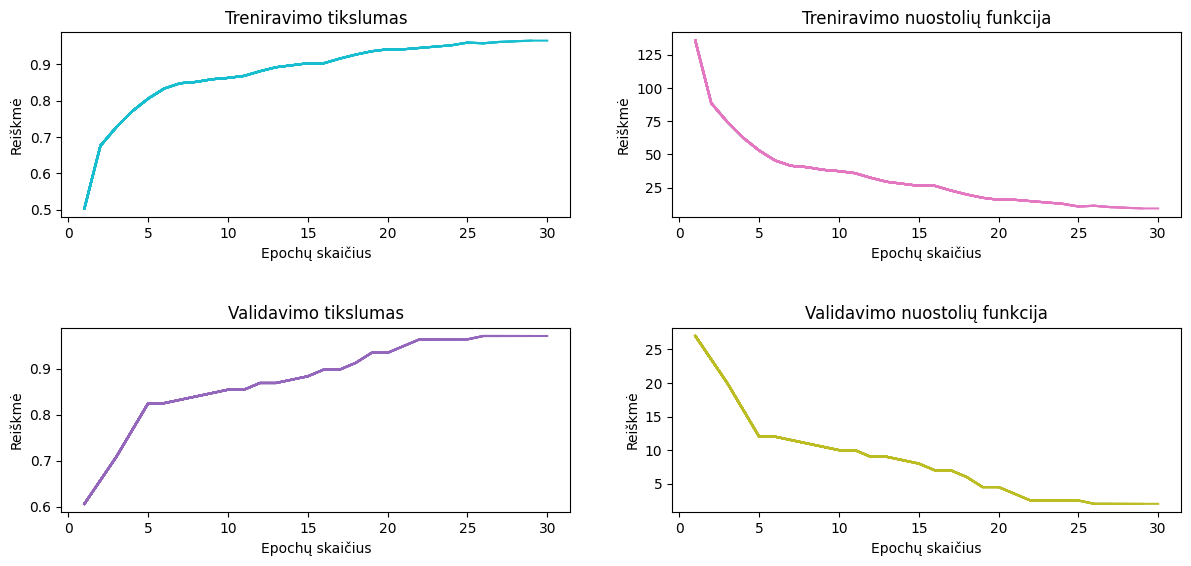
\includegraphics[scale=0.5]{img/2.png}
  \caption{Perceptrono mokymas naudojant krūties vėžio
   duomenų rinkinį ir slenkstinę aktyvacijos funkciją.
   Epochų skaičius: 30, mokymosi greitis: 0,001}
  \label{img:cancer-heaviside}
\end{figure}


\begin{figure}[H]
  \centering
  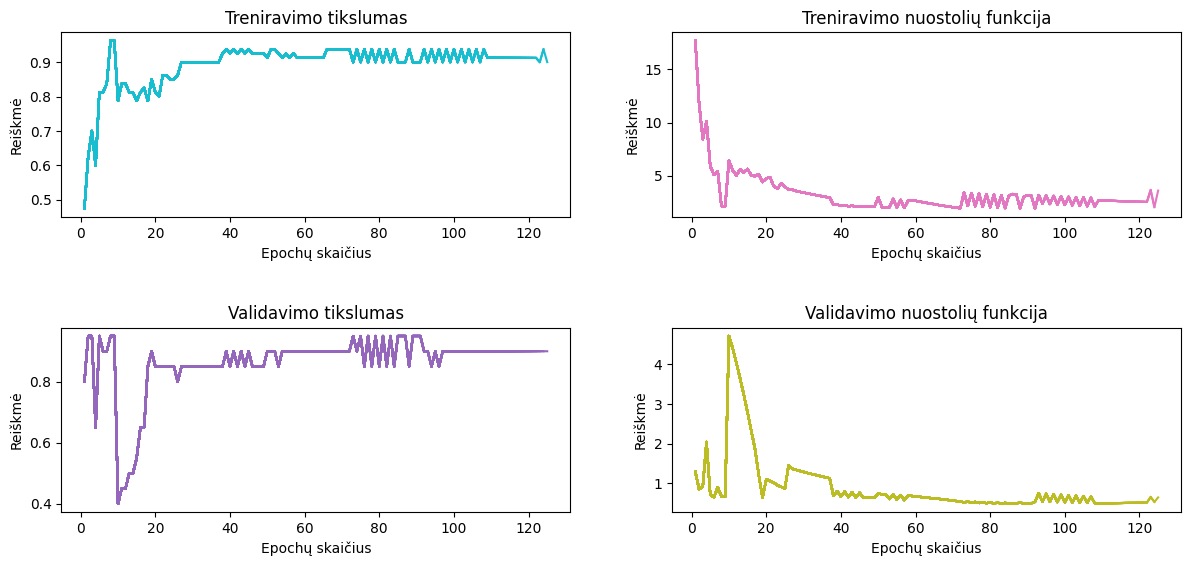
\includegraphics[scale=0.5]{img/3.png}
  \caption{Perceptrono mokymas naudojant irisų
   duomenų rinkinį ir sigmoidinę aktyvacijos funkciją.
   Epochų skaičius: 125, mokymosi greitis: 0,1}
  \label{img:iris-sigmoid}
\end{figure}


\begin{figure}[H]
  \centering
  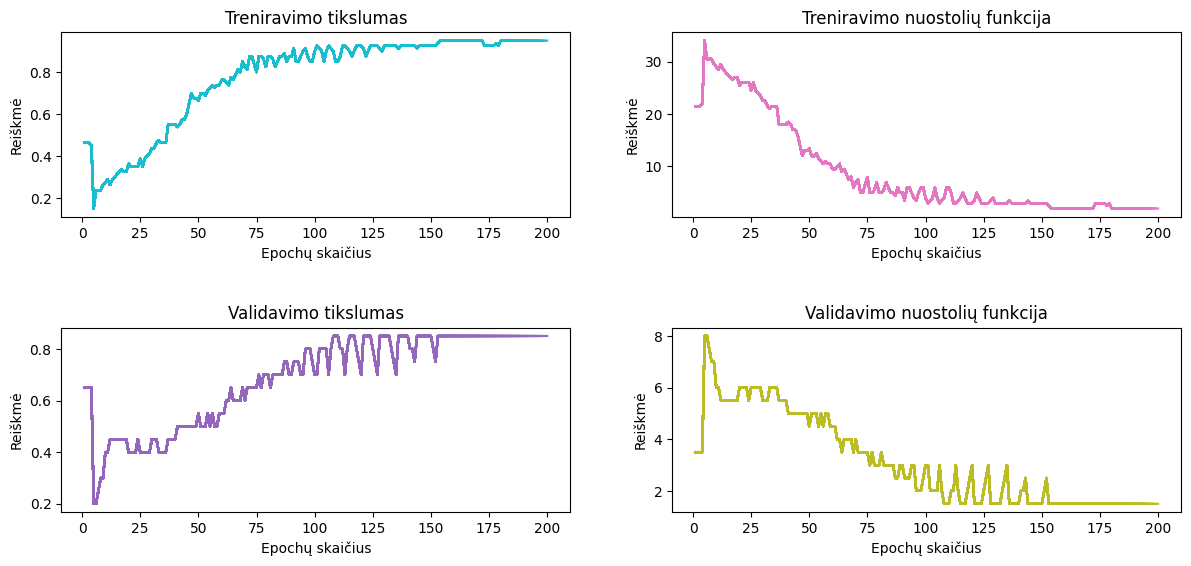
\includegraphics[scale=0.5]{img/4.png}
  \caption{Perceptrono mokymas naudojant irisų
   duomenų rinkinį ir slenkstinę aktyvacijos funkciją.
   Epochų skaičius: 200, mokymosi greitis: 0,001}
  \label{img:iris-heaviside}
\end{figure}


% Please add the following required packages to your document preamble:
% \usepackage{multirow}
\begin{table}[]
  \centering
  \caption{Krūties vėžio duomenų rinkinio rezultatai, epochų skaičius = 100}{
  \begin{tabular}{|c|cc|cc|}
  \hline
  \multirow{2}{*}{\textbf{Mokymosi greitis}} & \multicolumn{2}{c|}{\textbf{Tikslumas}}                         & \multicolumn{2}{c|}{\textbf{Nuostolių f. reikšmė}}              \\ \cline{2-5} 
                                             & \multicolumn{1}{c|}{\textbf{Treniravimo}} & \textbf{Validavimo} & \multicolumn{1}{c|}{\textbf{Treniravimo}} & \textbf{Validavimo} \\ \hline
  0,001                                      & \multicolumn{1}{c|}{0,95}                 & 0,97                & \multicolumn{1}{c|}{61,35}                & 15,44               \\ \hline
  0,01                                       & \multicolumn{1}{c|}{0,96}                 & 0,96                & \multicolumn{1}{c|}{19,6}                 & 4,88                \\ \hline
  1                                          & \multicolumn{1}{c|}{0,95}                 & 0,97                & \multicolumn{1}{c|}{10,98}                & 1,99                \\ \hline
  \end{tabular}}
  \label{tab:e-100-cancer-sig}
  \end{table}

% Please add the following required packages to your document preamble:
% \usepackage{multirow}
\begin{table}[]
  \centering
  \caption{Krūties vėžio duomenų rinkinio rezultatai, epochų skaičius = 10}{
  \begin{tabular}{|c|cc|cc|}
  \hline
  \multirow{2}{*}{\textbf{Mokymosi greitis}} & \multicolumn{2}{c|}{\textbf{Tikslumas}}                         & \multicolumn{2}{c|}{\textbf{Nuostolių f. reikšmė}}              \\ \cline{2-5} 
                                             & \multicolumn{1}{c|}{\textbf{Treniravimo}} & \textbf{Validavimo} & \multicolumn{1}{c|}{\textbf{Treniravimo}} & \textbf{Validavimo} \\ \hline
  0,001                                      & \multicolumn{1}{c|}{0,82}                 & 0,79                & \multicolumn{1}{c|}{40,80}                & 10,79               \\ \hline
  0,01                                       & \multicolumn{1}{c|}{0,93}                 & 0,92                & \multicolumn{1}{c|}{35,60}                & 9,79                \\ \hline
  1                                          & \multicolumn{1}{c|}{0,94}                 & 0,95                & \multicolumn{1}{c|}{16,39}                & 3,53                \\ \hline
  \end{tabular}}
  \label{tab:e-10-cancer-sig}
  \end{table}

  % Please add the following required packages to your document preamble:
% \usepackage{multirow}
\begin{table}[]
  \centering
  \caption{Irisų duomenų rinkinio rezultatai, epochų skaičius = 100}{
  \begin{tabular}{|c|cc|cc|}
  \hline
  \multirow{2}{*}{\textbf{Mokymosi greitis}} & \multicolumn{2}{c|}{\textbf{Tikslumas}}                         & \multicolumn{2}{c|}{\textbf{Nuostolių f. reikšmė}}              \\ \cline{2-5} 
                                             & \multicolumn{1}{c|}{\textbf{Treniravimo}} & \textbf{Validavimo} & \multicolumn{1}{c|}{\textbf{Treniravimo}} & \textbf{Validavimo} \\ \hline
  0,001                                      & \multicolumn{1}{c|}{0,85}                 & 0,85                & \multicolumn{1}{c|}{6,55}                 & 1,63                \\ \hline
  0,01                                       & \multicolumn{1}{c|}{0,91}                 & 0,85                & \multicolumn{1}{c|}{6,31}                 & 1,63                \\ \hline
  1                                          & \multicolumn{1}{c|}{0,94}                 & 0,9                 & \multicolumn{1}{c|}{2,25}                 & 1,00                \\ \hline
  \end{tabular}}
  \label{tab:e-100-iris-sig}
  \end{table}


% Please add the following required packages to your document preamble:
% \usepackage{multirow}
\begin{table}[]
  \centering
  \caption{Irisų duomenų rinkinio rezultatai, epochų skaičius = 10}{
  \begin{tabular}{|c|cc|cc|}
  \hline
  \multirow{2}{*}{\textbf{Mokymosi greitis}} & \multicolumn{2}{c|}{\textbf{Tikslumas}}                         & \multicolumn{2}{c|}{\textbf{Nuostolių f. reikšmė}}              \\ \cline{2-5} 
                                             & \multicolumn{1}{c|}{\textbf{Treniravimo}} & \textbf{Validavimo} & \multicolumn{1}{c|}{\textbf{Treniravimo}} & \textbf{Validavimo} \\ \hline
  0,001                                      & \multicolumn{1}{c|}{0,68}                 & 0,8                 & \multicolumn{1}{c|}{8,12}                 & 1,99                \\ \hline
  0,01                                       & \multicolumn{1}{c|}{0,56}                 & 0,7                 & \multicolumn{1}{c|}{9,59}                 & 2,25                \\ \hline
  1                                          & \multicolumn{1}{c|}{0,81}                 & 0,5                 & \multicolumn{1}{c|}{7,19}                 & 4,99                \\ \hline
  \end{tabular}}
  \label{tab:e-10-iris-sig}
  \end{table}

\section{Išvados}
Didinant epochų skaičių, didėja klasifikavimo tikslumas. Esant per dideliam
epochų skaičiui modelis tampa permokytu. Ženklaus skirtumo tarp slenkstinės
ir sigmoidinės funkcijų nepastebėta. Tendencijų kintant mokymosi greičiui nerasta,
tačiau palyginimai atlikti nefiksuojant svorių inicializavimo. Siekiant labiau ištirti
mokymosi greičio įtaką neurono mokymuisi, reikia pakartoti eksperimentą ne tik su
fiksuotu epochų skaičiumi, bet ir fiksuotais pradiniais svoriais.

\end{document}
